\section{Uppgift 9}\label{uppgift-9}

\subsection{Instruktioner}
\begin{verbatim}
9. Skriv ett program som summerar alla jämna tal från och med 0 t.o.m 200 med
   hjälp av en while-sats och sedan skriver ut denna summa. Skriv sedan två
   program till som utför samma sak, men som istället använder sig av en do-
   resp en for-sats. Observera att du ska skriva de tre programmen utan att
   använda någon if-sats inne i iterations-satserna.
\end{verbatim}

\subsection{Lösning}
\subsubsection{Funktion}
% TODO: Funktion på %9.
\subsection{Kommentar}
% TODO: Kommentar på #9.

\subsubsection{Källkod}\label{uppgift-9_src}
%\begin{listing}[H]
    \inputminted[linenos]{java}{src/Lab1Uppg09.java}
    \caption{Lab1Uppg09.java}
    \label{Uppg9src}
%\end{listing}

\subsubsection{Skärmdump}
\begin{figure}[htbp]
    \centering
        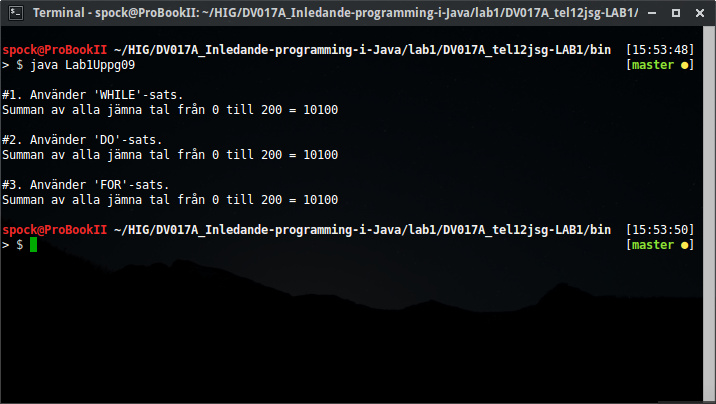
\includegraphics[width=\linewidth]{img/09.png}
    \caption{Körning av koden till Uppgift \ref{uppgift-9}}
    \label{fig:screenshot-09}
\end{figure}
